% -*- root: ../main.tex -*-
\chapter{Analisi dello spazio del problema}

	\section{Knowledge crunching}
    Per poter fare un'analisi soddisfacente è fondamentale avere una buona conoscenza del \textbf{dominio} e della sua \textbf{terminologia}, cosa che, se fatta in autonomia, potrebbe richiedere parecchio tempo. Per questo motivo è importante \textbf{collaborare} con gli \textbf{esperti di dominio}, che aiutano a comprendere i componenti del dominio, le dinamiche, i termini tecnici e gli aspetti critici.
    Il \textbf{knowledge crunching} è il percorso che porta chi deve realizzare il sistema ad avere una \textbf{migliore comprensione} non solo di \textbf{quanto} deve essere fatto, ma del \textbf{perché}, permettendo di non fermarsi alle \textbf{specifiche}, ma di capirne il \textbf{senso}. 
    
    \subsection{Sessioni}
	Nel nostro caso le sessioni di \textbf{knowledge crunching} sono state svolte interpellando un \textbf{esperto di dominio} per via telematica.
	\begin{itemize}
	    \item \textbf{Prima sessione:} nella prima sessione, il \textbf{colloquio} con l'esperto ha permesso al team di comprendere:
	    \begin{itemize}
	        \item gli aspetti principali della \textbf{gestione} del canile;
	        \item le \textbf{figure} coinvolte;
	        \item i \textbf{ruoli} presenti all'interno del canile;
	        \item le \textbf{mansioni} che vengono svolte quotidianamente;
	        \item i \textbf{processi di gestione}.
	    \end{itemize}
	    Queste conoscenze hanno permesso di dare il \textbf{kick-off} al progetto.

	    \item \textbf{Sessioni successive:} successivamente il processo è stato continuo, sono stati svolti degli \textbf{incontri periodici} per:
	    \begin{itemize}
	        \item controllare che il progetto proseguisse nella direzione sperata;
	        \item \textbf{sciogliere} alcuni \textbf{dubbi} sorti in corso d'opera;
	        \item \textbf{verificare} la corretta \textbf{comprensione} di alcuni concetti chiave. 
	    \end{itemize}
	\end{itemize}
    
    \subsection{Svolgimento}
    \subsubsection{Comunicazione}
	Data l'ovvia problematicità nell'incontrarsi, la comunicazione è stata gestita da remoto, utilizzando le seguenti piattaforme:
	\begin{itemize}
	    \item \textbf{Telegram}, per chiamate vocali e brevi chiarimenti
	    \item \textbf{Discord}, per la condivisione schermo con gli artefatti visuali
	\end{itemize}
	Durante le interazioni sono state create multiple \textbf{rappresentazioni visuali} a guida e supporto della conversazione. 
	
	\subsubsection{Percorso}
	\begin{itemize}
	    \item Il gruppo parlando con il \textbf{responsabile del canile} (il maggiore esperto del dominio) ha \textbf{indagato} con maggiore enfasi i concetti necessari per la creazione di un \textbf{buon software}, tralasciando dettagli \textbf{pleonastici}. 
	    \item Il \textbf{focus} è stato su capire quello che serve per lo sviluppo di un software che soddisfi le \textbf{reali necessità} del cliente. I dettagli su cui l'esperto del dominio ricadeva spesso, infatti, hanno rivelato dove le energie dovessero essere maggiormente spese. 
	    \item In questo caso gli \textbf{esperti} del dominio sono anche i \textbf{clienti}. Questi ultimi forniscono il \textbf{problem-space}, mentre i primi forniscono il \textbf{solution-space}.
	    \end{itemize}
	
	Per la comprensione degli obbiettivi di più alto business value, si è costruita in maniera interattiva e collaborativa un'impact map, sotto la supervisione di team, scrum master e product-owner. L'uso di questo diagramma mira a mantenere un livello non troppo formale da risultare incomprensibile agli estranei al dominio, ma nemmeno totalmente informale, perdendo efficacia comunicativa. 
	
	%IMPACT MAP DIAGRAM
    \begin{figure}[ht]
        \caption{Impact-map obbiettivi business}
        \centering
        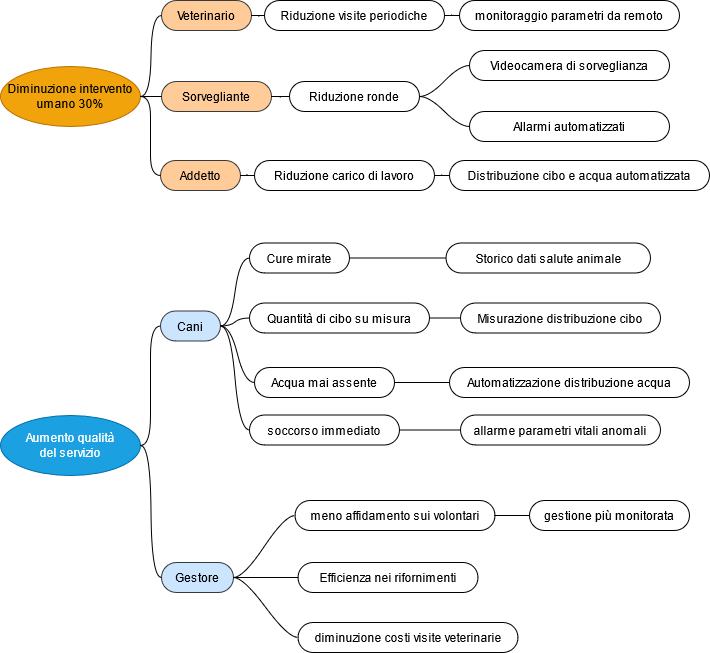
\includegraphics[width=1\textwidth]{DrawIo/impactMap.png}
    \end{figure}

    Il risultato ha portato in evidenza i due principali obbiettivi di business, evidenziando in maniera chiara la loro suddivisione, e le soluzioni per raggiungere i risulati attesi.
    
    Con una visone d'insieme leggermente più definita, ci siamo cimentati nella stesura delle \textbf{user stories} per ogni ruolo. Dalla moltitudine emersa, sono state identificate, cercando di seguire i requisiti di business individuati,  le più calzanti, legate ad ogni obiettivo dell'\textbf{impact map}.

	La definizione delle user-stories ha portato naturalmente a indagare il significato di alcuni termini usati. Questo ha spinto subito allo sviluppo concorrente di un ubiquitous language per i vocaboli più importanti. Questo è stato poi continuamente raffinato durante i successivi meeting. 
	Nel prossimo capitolo viene analizzato questo processo. 
    
	\section{Definizione Ubiquitous Language}	
	L'Ubiquitous Language deve essere espresso nel modello di dominio, infatti unisce le persone del team di progetto.
    Lo scopo è eliminare le imprecisioni e le contraddizioni degli esperti di dominio, non è infatti imposto da questi, ma raggiunto collaborativamente.
    L'Ubiquitous Language si evolve nel tempo, non è definito interamente in una sola riunione, i concetti spesso si aggiungono, vengono sviscerati e partecipano nella comprensione del dominio. Infatti quelli che non fanno parte dell'Ubiquitous Language devono essere rifiutati.
    
    \newcounter{tabellaDrawIo}
    \setcounter{tabellaDrawIo}{1} %1=True, usa la tabella di DrawIo
    \ifthenelse{\value{tabellaDrawIo}=1} {
    
        %TABELLA UBIQUITOUS LANGUAGE
        \begin{figure}[ht]
            \caption{Tabella ubiquitous language}
            \centering
            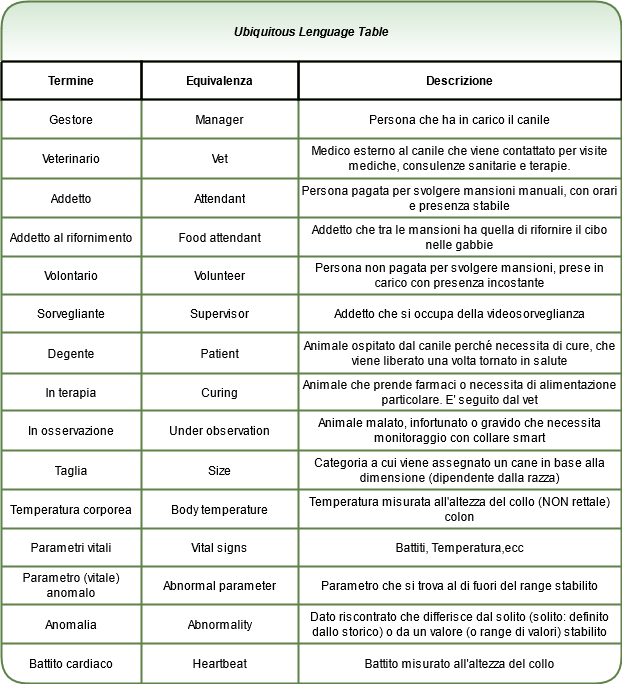
\includegraphics[width=0.9\textwidth]{DrawIo/ubiquitousLanguage.png}
        \end{figure}
        
    }{ %else
    
        %tab prova
        \begin{tcolorbox}[tab2,tabularx={c||c|Y},title=Ubiquitous Language,boxrule=0.5pt]
            Termine & Equivalenza     & Descrizione     \\\hline\hline
            Gestore   & Manager & Persona che ha in carico il canile  \\
            Veterinario & Vet & Medico esterno al canile che viene contattato per visite mediche consulenze sanitarie e terapie \\
            Blue  & 3000.00 & 4000.00  \\\hline\hline
            Sum   & 6000.00 & 9000.00 
        \end{tcolorbox}
    
    } %close else
    
    
    \subsection{Glossario degli incarichi}

        La definizione di un organigramma generico che individua le figure che operano all'interno del canile e le loro interazioni è stata raggiunta in seguito all'analisi della struttura gerarchica dei due canili che sono stati interpellati in qualità di esperti del dominio. Si è cercato di cogliere gli aspetti comuni e di utilizzare le differenze come base per elaborare un modello che interiorizzasse un livello di astrazione tale da permettere al sistema che ne deriverà di adattarsi a un qualsiasi canile. Il seguente organigramma più che sulle effettive figure nasce dall'astrazione dei principali ruoli che esse ricoprono. Questa scelta è dovuta al fatto che dallo \textbf{storytelling} di entrambi i canili è emerso un certo grado di caoticità nella suddivisione delle mansioni che spesso, per necessità, tendono ad essere svolte da chi si trova lì in quel momento. Da ciò deriva che, più o meno, tutti i dipendenti dovrebbero essere in grado di fare tutto anche se, nella pratica, una suddivisione dei ruoli esiste, seppure non netta. Ciò accade anche per le mansioni di tipo burocratico, la cui suddivisione avviene mediante accordo verbale tra i colleghi e non in base a ruoli scritti. De facto, si sa che a occuparsi di un certo tipo di pratiche è una determinata persona, ma, sulla carta, i dipendenti hanno lo stesso identico contratto.
        
        I canili da noi consultati, tuttavia, sono di piccole/medie dimensioni. Più il canile è grande, più la gestione risulta complicata e di conseguenza diventa sempre più forte la necessità di definire delle responsabilità. Per questo motivo il seguente organigramma è stato costruito in modo da suddividere secondo criteri logici e concettuali le mansioni, mappandole con delle figure, ma permettendo alla stessa persona di inglobarne più di una.
        
            	    %Organization Chart - Organigramma
        \begin{figure}[ht]
            \caption{Organization Chart}
            \centering
            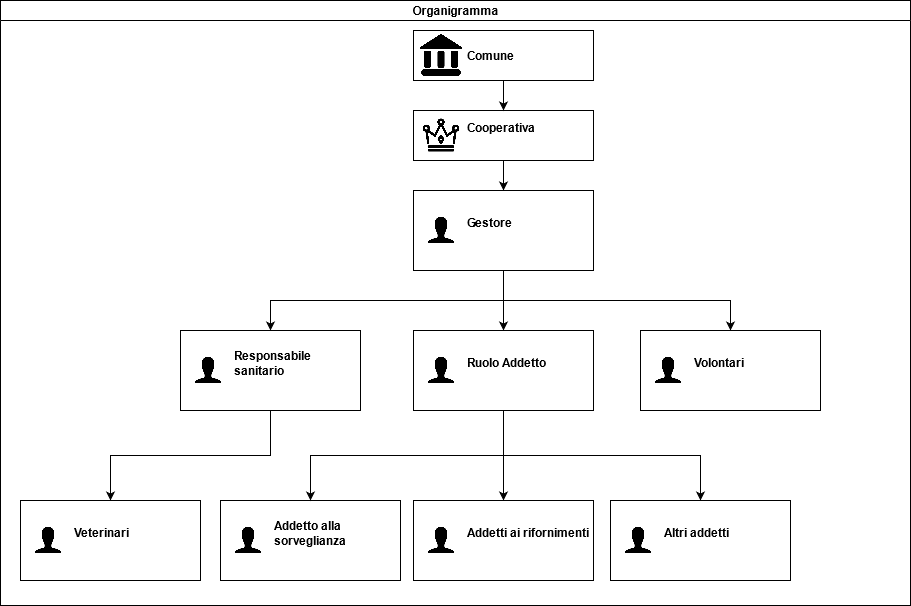
\includegraphics[width=0.9\textwidth]{DrawIo/organizationChart.png}
        \end{figure}